Dans ce chapitre, nous décrivons la mise en œuvre des analyses statiques
précédentes. Nous commençons par un tour d'horizon des représentations
intermédiaires possibles, avant de décrire celle retenue : Newspeak. La chaîne
de compilation est explicitée, partant de C pour aller au langage impératif
décrit dans le chapitre~\ref{cha:typbase}. Enfin, nous donnons les détails d'un
algorithme d'inférence de types à la Hindley-Milner, reposant sur l'unification
et le partage de références.

\section{Langages intermédiaires}

Le langage C \cite{KandR,AnsiC} a été conçu pour être une sorte d'assembleur
portable, permettant décrire du code indépendamment de l'architecture sur
laquelle il sera compilé. Historiquement, c'est il a permis de créer Unix, et
ainsi de nombreux logiciels bas niveau sont écrits en C. En particulier, il
existe des compilateurs de C vers les différents langages machine pour à peu
près toutes les architectures.

\begin{figure}
  \centering

  \begin{tikzpicture}
[>=latex]
  \node (me) {Langage intermédiaire};
  \node[ above left of=me, xshift=-4cm] (fe1) {Langage source 1};
  \node[ below left of=me, xshift=-4cm] (fe2) {Langage source 2};
  \node[above right of=me, xshift=4cm] (be1) {Langage destination 1};
  \node[below right of=me, xshift=4cm] (be2) {Langage destination 2};

  \draw[->] (fe1) -- (me);
  \draw[->] (fe2) -- (me);

  \draw[->] (me) -- (be1);
  \draw[->] (me) -- (be2);

  \path (me) edge [loop below] node {Optimisations, analyses} (me);

  \coordinate (legbase) at ($ (me) + (0,-2cm) $);

  \draw[bigbrace] ($ (me.south east |- legbase) + (-2mm, 0) $)
               to node [yshift=-5mm] {Middle-end}
                  ($ (me.south west |- legbase) + (2mm, 0) $);
  \draw[bigbrace] (me.south west |- legbase)
               to node [yshift=-5mm]{Front-end}
                  (fe2.south west |- legbase);
  \draw[bigbrace] (be2.south east |- legbase)
               to node [yshift=-5mm]{Back-end}
                  (me.south east |- legbase);
\end{tikzpicture}


  \caption{Décomposition d'un compilateur : front-ends, middle-end, back-ends}
  \label{fig:middle-end}
\end{figure}

Lors de l'écriture d'un compilateur, on a besoin d'un langage intermédiaire qui
fasse l'intermédiaire entre \emph{front-end} et \emph{back-end}
(figure~\ref{fig:middle-end}). Depuis ce langage on doit pouvoir exprimer des
transformations intermédiaires sur cette représentation (analyses sémantiques,
optimisations, etc), mais aussi compiler ce langage vers un langage machine.

L'idée de prendre C comme langage intermédiaire est très séduisante, mais
malheureusement sa sémantique est trop complexe et trop peu spécifiée. Il est
donc judicieux d'utiliser un langage plus simple à cet effet. Dans de nombreux
projets, des sous-ensembles de C ont été définis pour aller dans ce sens.

\subsubsection{Critères}

Les critères à évaluer sont les suivants :

\begin{itemize}
\item
  Forme (textuel / langage d'implem) : Quelle est la représentation du
  langage? Est-ce une bibliothèque (si oui, dans quel langage) a-t'il
  une forme textuelle (si oui, pour quels langages des \emph{parsers}
  existent ils).
\item
  Maturité : Le langage a-t'il ``fait ses preuves'' ? Est-il susceptible
  de changer ?
\item
  Tools
\item
  Support
\item
  Scope (analyse / compil) : pour quel type d'utilisation a-t'il été
  conçu ?
\item Expressivité : Peut-on compiler ``tout C'' ?
\item Orthogonalité
\item Typage
\item Sémantique existante
\end{itemize}

\subsubsection{Langages}

\begin{itemize}
\item
  GIMPLE\cite{gcc-gimple} : la représentation intermédiaire utilisée par GCC.
\item
  LLVM\cite{llvm-pres} : un backend de compilateur développé par Apple.
\item
  Cmm (OCaml) : cf. \texttt{asmcomp/cmm.mli}
\item
  CIL\cite{NeculaCil} \link{kerneisCil} utilisé par Frama-C, Compcert.
\item
  Clight\cite{cfront} : Utilisé dans Compcert (front-end)
\item
  Cminor\cite{cminorSL}, utilisé dans Compcert (middle-end).
\item
  Cminusminus \cite{spjcmm} \link{cmm}
\item
  Newspeak\cite{newspeak}, décrit dans la section~\ref{sec:npk}.
\end{itemize}

\def\ilfeatfna{\footnote{C : Compilation, A : Analyse}}

\begin{tabular}{| l || l | l | l | l | l | l |}
\hline
Nom           & Langage hôte    & Description       & But\ilfeatfna & Langage source                   &  Sémantique & Types \\ \hline \hline
C             & Texte           & \cite{AnsiC}      & C             & C                                &  Non        & Oui   \\ \hline
GIMPLE        & C               & \cite{gcc-gimple} & C             & C + extensions, C++, Ada, \ldots &  Non        & Non   \\ \hline
LLVM          & C++             & \cite{llvm-pres}  & C             & C + extensions, C++, Ada, \ldots &             & Oui   \\ \hline
Cminusminus   & Texte           & \cite{spjcmm}     & C             &                                  &             & Oui   \\ \hline
Cmm (Haskell) & Texte / Haskell &                   & C             &                                  &             &       \\ \hline
Cmm (OCaml)   & OCaml           &                   & C             &                                  &             &       \\ \hline
CIL           & OCaml           & \cite{NeculaCil}  & A             &                                  &             &       \\ \hline
Clight        & Coq             & \cite{cfront}     & C/A           &                                  &  Oui        & Oui   \\ \hline
Cminor        & Coq             & \cite{cminorSL}   & C/A           &                                  &  Oui        & Oui   \\ \hline
Newspeak      & Ocaml           & \cite{newspeak}   & A             &                                  &  Oui        & Oui   \\ \hline
\end{tabular}

% vim: textwidth=0


\section{Newspeak}
\label{sec:npk}

\section{Chaîne de compilation}

\begin{figure}
  \centering
  \begin{tikzpicture}\shorthandoff{!}
\tikzstyle{file}=[draw, shape=rectangle, node distance=2.2cm, minimum
height=1cm, shade, top color=white,
    bottom color=blue!50!black!20, draw=blue!40!black!60, very thick];

\node [file] (c1) {\textcolor{black}{.c}};
\node [file, below of=c1] (c2) {\textcolor{black}{.c}};
\node [node distance=2.2cm, below of=c2] (c3) {};

\node [file, minimum height=0, node distance=5mm, above of=c3,draw] (c3b) {.adb};
\node [file, minimum height=0, node distance=5mm, below of=c3,draw] (c3s) {.ads};

\path (c3b.north west) ++(-3mm,3mm) [draw,dotted] rectangle ($(c3s.south east)+(3mm,-3mm)$);

\node [below of=c3, node distance=2.2cm] (c4){};

\node [file, right of=c1] (cc1) {\textcolor{black}{.c}};
\node [file, right of=c2] (cc2) {\textcolor{black}{.c}};
\node [node distance=2.2cm, right of=c3] (cc3) {};

\node [below of=cc3, node distance=2.2cm](cc4){};

\draw[->] (c1) -- node[above] {{\tiny \ttfamily gcc -E}} (cc1);
\draw[->] (c2) -- (cc2);

\node [file, right of=cc1] (no1) {\textcolor{black}{.no}};
\node [file, right of=cc2] (no2) {\textcolor{black}{.no}};
\node [file, right of=cc3] (no3) {\textcolor{black}{.no}};

\node [below of=no3, node distance=2.2cm](no4){};

\draw[->] (cc1) -- node[above] {{\tiny \ttfamily c2newspeak -c}} (no1);
\draw[->] (cc2) --  (no2);

\draw[->] ($ (c3b.north east)!0.5!(c3s.south east) + (3mm,0) $) -- node[above] {\tiny \ttfamily ada2newspeak -c} (no3);


\node [file, right of=no2] (npk) {\textcolor{black}{.npk}};

\node [right of=no3, node distance=2.2cm](npk2){};
\node [right of=no4, node distance=2.2cm](npk3){};

\node[draw, ellipse, right of=no2, minimum height=3cm]{};

\draw[->] (no1) -- node {} (npk);
\draw[->] (no2) -- node[above] {{\tiny \ttfamily c2newspeak}} (npk);
\draw[->] (no3) -- node {} (npk);


\node [file, right of=npk](warn) {\textcolor{black}{.warn}};

\node [right of=npk3, node distance=3cm](analyser2){};

\draw[->] (npk) -- node[above] {{\tiny \ttfamily penjili}} (warn);

\draw[->] (c4)   -- node[above, text depth=3pt] {\footnotesize Pr\'etraitement} (cc4);
\draw[->] (cc4)  -- node[above, text depth=3pt] {\footnotesize Compilation} (no4);
\draw[->] (no4)  -- node[above, text depth=3pt] {\footnotesize \'Edition de liens} (npk3);
\draw[->] (npk3) -- node[above, text depth=3pt] {\footnotesize Analyse} (analyser2);
\end{tikzpicture}

  \caption{Compilation depuis Newspeak}
  \label{fig:compil-npk}
\end{figure}

La compilation vers C est faite en trois étapes (figure~\ref{fig:compil-npk}) :
prétraitement du code source, compilation de C prétraité vers \newspeak{}, puis
compilation de \newspeak{} vers ce langage.

\subsection{Prétraitement}

\ctonewspeak{} travaillant uniquement sur du code prétraité (dans directives de
préprocesseur), la première étape consiste donc à faire passer le code par \cpp.

\subsection{Compilation (levée des ambigüités)}

Cette passe est réalisée par l'utilitaire \ctonewspeak{}. L'essentiel de la
compilation consiste à mettre à plat les définition de types, et à simplifier le
flôt de contrôle. C en effet propose de nombreuses constructions ambigües ou
redondantes.

Au contraire, \newspeak{} propose un nombre réduit de constructions. Rappelons
que le but de ce langage est de faciliter l'analyse statique : des constructions
orthogonales permettent donc d'éviter la duplication de règles sémantique, ou de
code lors de l'implémentation d'un analyseur.

Par exemple, plutôt que de fournir une boucle while, une boucle do/while et une
boucle for, \newspeak{} fournit une unique boucle \npkWhile{}. La sortie de
boucle est compilée vers un \npkGoto{}, qui est toujours un saut vers l'avant
(similaire à un "break" généralisé).

La sémantique de \newspeak{} et la traduction de C vers \newspeak{} sont
décrites dans \cite{newspeak}. En ce qui concerne l'élimination des sauts vers
l'arrière, on peut se référer à \cite{goto}.

\subsection{Annotations}

\newspeak{} a de nombreux avantages, mais pour une analyse par typage il est
trop bas niveau. Par exemple, dans le code suivant

\begin{Verbatim}[commandchars=\\\{\}]
\PY{k}{struct} \PY{n}{s} \PY{p}{\PYZob{}}
    \PY{k+kt}{int} \PY{n}{a}\PY{p}{;}
    \PY{k+kt}{int} \PY{n}{b}\PY{p}{;}
\PY{p}{\PYZcb{}}\PY{p}{;}

\PY{k+kt}{int} \PY{n+nf}{main}\PY{p}{(}\PY{k+kt}{void}\PY{p}{)}
\PY{p}{\PYZob{}}
    \PY{k}{struct} \PY{n}{s} \PY{n}{x}\PY{p}{;}
    \PY{k+kt}{int} \PY{n}{y}\PY{p}{[}\PY{l+m+mi}{10}\PY{p}{]}\PY{p}{;}
    \PY{n}{x}\PY{p}{.}\PY{n}{b} \PY{o}{=} \PY{l+m+mi}{1}\PY{p}{;}
    \PY{n}{y}\PY{p}{[}\PY{l+m+mi}{1}\PY{p}{]} \PY{o}{=} \PY{l+m+mi}{1}\PY{p}{;}
    \PY{k}{return} \PY{l+m+mi}{0}\PY{p}{;}
\PY{p}{\PYZcb{}}
\end{Verbatim}


\subsection{Implantation de l'algorithme de typage}

Commençons par étudier le cas du lambda-calcul simplement typé
(figure~\ref{fig:stlc}).

\begin{figure}

\begin{align*}
\gramdef{Expressions}{e}
  { n              }{Entier}
  { d              }{Flottant}
  { x              }{Variable}
  { λ x . e        }{Abstraction}
  { e_1~e_2        }{Application}
  { (e_1, e_2)     }{Couple}
  { \textrm{fst}~e }{Projection gauche}
  { \textrm{snd}~e }{Projection droite}
  {END}
\\
\\
\gramdef{Types}{t}
  {  \tInt          }{Entier}
  {  \tFloat        }{Flottant}
  { t \rightarrow t }{Fonction}
  { t \times t      }{Produit}
  {END}
\\
\\
\gramdef{Contextes}{Γ}
  { ε     }{Contexte vide}
  { Γ,x:t }{Extension}
  {END}
\end{align*}

\ruleheader{$Γ ⊢ e : t$}
\begin{mathpar}
\irule{Int}{ }{Γ⊢n:\tInt}

\irule{Float}{ }{Γ⊢d:\tFloat}

\irule{Var}{(x:t)∈Γ}{Γ⊢x:t}

\irule{Abs}{Γ,(x:t_1)⊢ e : t_2}{Γ⊢ λx.e:t_1 \rightarrow t_2}

\irule{App}{Γ⊢e:t_1 \rightarrow t_2 \\ Γ ⊢ e' : t_1}{Γ ⊢ e~e' : t_2}

\irule{Proj-g}{Γ⊢x:t_1\times t_2}{Γ⊢\textrm{fst}~x:t_1}

\irule{Proj-d}{Γ⊢x:t_1\times t_2}{Γ⊢\textrm{snd}~x:t_2}

\irule{Tup}{Γ⊢x:t_1 \\ Γ⊢y:t_2}{Γ⊢(x,y):t_1 \times t_2}
\end{mathpar}


\caption{Lambda calcul simplement typé avec entiers, flottants et couples}
\label{fig:stlc}

\end{figure}

Prenons l'exemple de la fonction suivante\footnote{ On suppose que \texttt{plus}
est une fonction de l'environnement global qui a pour type $\tInt \rightarrow
\tInt \rightarrow \tInt$.} :

\[
f = λx.λy. \textrm{plus} (\textrm{plus} (\textrm{fst} x) (\textrm{snd} x)) y
\]

Informellement, on voit que puisque \texttt{fst} et \texttt{snd} sont appliqués
à \texttt{x}, ce doit être un tuple. En outre on additionne ces deux composantes
ensemble, donc elles doivent être de type \tInt (et le résultat aussi). Par le
même argument, \texttt{y} doit aussi être de type \tInt. En conclusion,
\texttt{x} est de type $\tInt \times \tInt$ et \texttt{y} de type $\tInt$, donc
f est de type $\tInt \times \tInt \rightarrow \tInt \rightarrow \tInt$.

Mais comment faire pour implanter cette analyse ? En fait le système de types de
la figure~\ref{fig:stlc} a une propriété particulièrement intéressante : chaque
forme syntaxique (variable, abstraction, etc) est en conclusion d'exactement une
règle de typage. Cela permet de toujours savoir quelle règle il faut appliquer
(c'est à rapprocher du fait qu'on peut déduire un analyseur syntaxique d'une
grammaire LL)

Partant du terme de conclusion ($f$), on peut donc en déduire un squelette
d'arbre d'inférence (figure~\ref{fig:inftree-rules})\footnote{Par souci de
clarté, les prémisses des applications de \textsc{(Var)} ne sont pas notées.}

\begin{figure} % {{{ Fig règles
\def\disptypeL#1{}
\def\disptypeR#1{}

\def\gammaXY{\ensuremath{Γ_2}}
\def\gammaX{\ensuremath{Γ_1}}
\def\gammaOneDef{\ensuremath{Γ^0, x\disptypeL{\tInt \times \tInt}, y\disptypeL{\tInt}}}
\def\gammaTwoDef{\ensuremath{Γ^0, x\disptypeL{\tInt \times \tInt}}}
\def\termFst#1{\ensuremath{\textrm{fst}~x}}
\def\termSnd#1{\ensuremath{\textrm{snd}~x}}
\def\fstx{\termFst{x}}
\def\sndx{\termSnd{x}}
\begin{mathpar}
\irule
  {Abs}
  {
    \irule
      {Abs}
      {
        \inferrule*[right=(App)]
          {
            \inferrule*[right=(Var), rightskip=4em]
              { }
              {\gammaXY ⊢ y
              \disptypeR{\tInt}
              }
            \\
            \inferrule*[right=(App),vdots=4em,leftskip=5em,rightskip=5em]
              {
                \inferrule*[right=(Var), leftskip=3em, rightskip=7em]
                  { }
                  {\gammaXY ⊢ \textrm{plus}
                  \disptypeR{\tInt \rightarrow \tInt \rightarrow \tInt}
                  }
                \\
                \inferrule*[right=(App),vdots=3em,leftskip=7em,rightskip=3em]
                  {
                    \inferrule*[right=(App), vdots=4em, rightskip=5em]
                      {
                        \inferrule*[right=(Var), rightskip=5em]
                          { }
                          {\gammaXY ⊢ \textrm{plus}
                          \disptypeR{\tInt \rightarrow \tInt \rightarrow \tInt}
                          }
                        \\
                        \inferrule*[right=(Proj-G), vdots=3em, leftskip=5em]
                          {
                            \irule
                              {Var}
                              { }
                              {\gammaXY ⊢ x
                              \disptypeR{\tInt \times \tInt}
                              }
                          }
                          {\gammaXY ⊢ \fstx
                          \disptypeR{\tInt}
                          }
                      }
                      {\gammaXY ⊢ \textrm{plus} (\fstx)
                      \disptypeR{\tInt \rightarrow \tInt}
                      }
                    \\
                    \inferrule*[right=(Proj-D), leftskip=5em, rightskip=4em]
                      {
                        \irule
                          {Var}
                          { }
                          {\gammaXY ⊢ x
                          \disptypeR{\tInt \times \tInt}
                          }
                      }
                      {\gammaXY ⊢ \sndx
                      \disptypeR{\tInt}
                      }
                  }
                  {\gammaXY ⊢ \textrm{plus} (\fstx) (\sndx)
                  \disptypeR{\tInt}
                  }
              }
              {\gammaXY ⊢ \textrm{plus} (\textrm{plus} (\fstx) (\sndx))
              \disptypeR{\tInt \rightarrow \tInt}
              }
          }
          {\gammaXY ⊢ \textrm{plus} (\textrm{plus} (\fstx) (\sndx)) y
          \disptypeR{\tInt}
          }
      }
      {\gammaX ⊢ λy. \textrm{plus} (\textrm{plus} (\fstx) (\sndx)) y
      \disptypeR{\tInt \rightarrow \tInt}
      }
  }
  {Γ_0 ⊢ λx.λy. \textrm{plus} (\textrm{plus} (\fstx) (\sndx)) y
  \disptypeR{\tInt \times \tInt \rightarrow \tInt \rightarrow \tInt}
  }
\end{mathpar}

\[\gammaX = \gammaTwoDef \qquad \gammaXY = \gammaOneDef\]


\caption{Arbre d'inférence : règles à utiliser}
\label{fig:inftree-rules}
\end{figure} % }}}

\begin{figure} % {{{ Fig full tree
\def\disptypeL#1{:#1}
\def\disptypeR#1{:#1}

\def\gammaXY{\ensuremath{Γ_2}}
\def\gammaX{\ensuremath{Γ_1}}
\def\gammaOneDef{\ensuremath{Γ^0, x\disptypeL{\tInt \times \tInt}, y\disptypeL{\tInt}}}
\def\gammaTwoDef{\ensuremath{Γ^0, x\disptypeL{\tInt \times \tInt}}}
\def\termFst#1{\ensuremath{\textrm{fst}~x}}
\def\termSnd#1{\ensuremath{\textrm{snd}~x}}
\def\fstx{\termFst{x}}
\def\sndx{\termSnd{x}}
\begin{mathpar}
\irule
  {Abs}
  {
    \irule
      {Abs}
      {
        \inferrule*[right=(App)]
          {
            \inferrule*[right=(Var), rightskip=4em]
              { }
              {\gammaXY ⊢ y
              \disptypeR{\tInt}
              }
            \\
            \inferrule*[right=(App),vdots=4em,leftskip=5em,rightskip=5em]
              {
                \inferrule*[right=(Var), leftskip=3em, rightskip=7em]
                  { }
                  {\gammaXY ⊢ \textrm{plus}
                  \disptypeR{\tInt \rightarrow \tInt \rightarrow \tInt}
                  }
                \\
                \inferrule*[right=(App),vdots=3em,leftskip=7em,rightskip=3em]
                  {
                    \inferrule*[right=(App), vdots=4em, rightskip=5em]
                      {
                        \inferrule*[right=(Var), rightskip=5em]
                          { }
                          {\gammaXY ⊢ \textrm{plus}
                          \disptypeR{\tInt \rightarrow \tInt \rightarrow \tInt}
                          }
                        \\
                        \inferrule*[right=(Proj-G), vdots=3em, leftskip=5em]
                          {
                            \irule
                              {Var}
                              { }
                              {\gammaXY ⊢ x
                              \disptypeR{\tInt \times \tInt}
                              }
                          }
                          {\gammaXY ⊢ \fstx
                          \disptypeR{\tInt}
                          }
                      }
                      {\gammaXY ⊢ \textrm{plus} (\fstx)
                      \disptypeR{\tInt \rightarrow \tInt}
                      }
                    \\
                    \inferrule*[right=(Proj-D), leftskip=5em, rightskip=4em]
                      {
                        \irule
                          {Var}
                          { }
                          {\gammaXY ⊢ x
                          \disptypeR{\tInt \times \tInt}
                          }
                      }
                      {\gammaXY ⊢ \sndx
                      \disptypeR{\tInt}
                      }
                  }
                  {\gammaXY ⊢ \textrm{plus} (\fstx) (\sndx)
                  \disptypeR{\tInt}
                  }
              }
              {\gammaXY ⊢ \textrm{plus} (\textrm{plus} (\fstx) (\sndx))
              \disptypeR{\tInt \rightarrow \tInt}
              }
          }
          {\gammaXY ⊢ \textrm{plus} (\textrm{plus} (\fstx) (\sndx)) y
          \disptypeR{\tInt}
          }
      }
      {\gammaX ⊢ λy. \textrm{plus} (\textrm{plus} (\fstx) (\sndx)) y
      \disptypeR{\tInt \rightarrow \tInt}
      }
  }
  {Γ_0 ⊢ λx.λy. \textrm{plus} (\textrm{plus} (\fstx) (\sndx)) y
  \disptypeR{\tInt \times \tInt \rightarrow \tInt \rightarrow \tInt}
  }
\end{mathpar}

\[\gammaX = \gammaTwoDef \qquad \gammaXY = \gammaOneDef\]


\caption{Arbre d'inférence complet}
\label{fig:inftree-full}
\end{figure} % }}}

Une fois à cette étape, on peut donner un nom à chaque type inconnu : $τ_1, τ_2,
\ldots$. L'utilisation qui en est faite permet de générer un ensemble de
contraintes d'unification. Par exemple, pour chaque application de la règle
\textsc{(App)} :

\[
\irule{App}{Γ⊢\ldots:τ_3 \\ Γ ⊢ \ldots : τ_1}{Γ ⊢ \ldots : τ_2}
\]

on doit déduire que $τ_3 = τ_1 \rightarrow τ_2$.

Ici $=$ est à prendre comme une contrainte d'égalité : partant d'un ensemble de
contraintes de la forme "type avec inconnue = type avec inconnue", on veut
obtenir une substitution "inconnue -> type concret".

Pour résoudre ces contraintes, on commence par les simplifier : si $τ_a
\rightarrow τ_b = τ_c \rightarrow τ_d$, alors $τ_a = τ_c$ et $τ_b = τ_d$. De
même si $τ_a \times τ_b = τ_c \times τ_d$. Au contraire, si $τ_a \rightarrow τ_b
= τ_c \times τ_d$, il est impossible d'unifier les types et il faut abandonner
l'inférence de types. D'autre cas sont impossibles, par exemple $\tInt = τ_1
\rightarrow τ_2$ ou $\tInt = \tFloat$.

Une fois ces simplifications réalisées, les contraintes restantes sont d'une des
formes suivantes :

\begin{itemize}
\item
  $τ_i = τ_i$. Il n'y a rien à faire, cette contrainte peut être supprimée.
\item
  $τ_i = τ_j$ avec $i \ne j$ : toutes les occurrences de $τ_j$ dans les autres
  contraintes peuvent être remplacées par $τ_i$. \todo{occurs check peut etre?}
\item
  $τ_i = x$ (ou $x = τ_i$) où $x$ est un type concret : idem.
\end{itemize}

\todo{C'est faux}

Une fois toutes les substitutions effectuées, on obtient un arbre de typage
correct (figure~\ref{fig:inftree-full}, donc un programme totalement inféré.

\begin{figure} % fig:unifpartage {{{

  \subfloat[][]{
  \label{fig:unifpartage:a}
  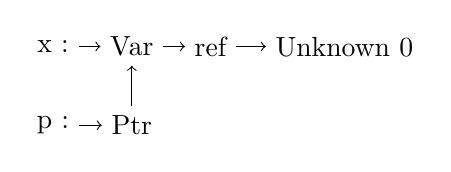
\begin{tikzpicture}
  \node               (var) {Var};
  \node[right of=var] (ref) {ref};
  \node[right of=ref, node distance=1.7cm] (u0) {Unknown 0};
  \node[below of=var] (ptr) {Ptr};
  \node[left of=var]  (x) {x :};
  \node[left of=ptr] (p) {p :};
  \draw[->] (x) -- (var);
  \draw[->] (p) -- (ptr);
  \draw[->] (ptr) -- (var);
  \draw[->] (var) -- (ref);
  \draw[->] (ref) -- (u0);
  \end{tikzpicture}
  }
  \subfloat[][]{
  \label{fig:unifpartage:b}
  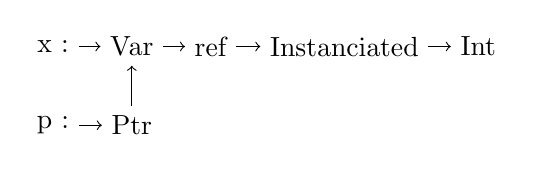
\begin{tikzpicture}
  \node               (var) {Var};
  \node[right of=var] (ref) {ref};
  \node[right of=ref, node distance=1.7cm] (u0) {Instanciated};
  \node[right of=u0, node distance=1.7cm] (ii) {Int};
  \node[below of=var] (ptr) {Ptr};
  \node[left of=var]  (x) {x :};
  \node[left of=ptr] (p) {p :};
  \draw[->] (x) -- (var);
  \draw[->] (p) -- (ptr);
  \draw[->] (ptr) -- (var);
  \draw[->] (var) -- (ref);
  \draw[->] (ref) -- (u0);
  \draw[->] (u0) -- (ii);
  \end{tikzpicture}
  }
  \subfloat[][]{
  \label{fig:unifpartage:c}
  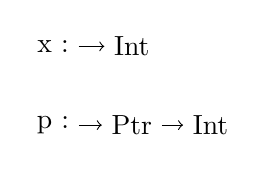
\begin{tikzpicture}
  \node               (var) {Int};
  \node[below of=var] (ptr) {Ptr};
  \node[left of=var]  (x) {x :};
  \node[left of=ptr] (p) {p :};
  \node[right of=ptr] (pi) {Int};
  \draw[->] (x) -- (var);
  \draw[->] (p) -- (ptr);
  \draw[->] (ptr) -- (pi);
  \end{tikzpicture}
  }

  \caption{Unification par partage}
  \label{fig:unifpartage}

\end{figure} % }}}

Plutôt que de modifier toutes les occurrences d'un type $τ_i$, on va affecter à
$τ_i$ la valeur du nouveau type.

L'implémentation de cet algorithme utilise le partage et les références
(figure~\ref{fig:unifpartage}).

D'abord \ref{fig:unifpartage:a}, ensuite \ref{fig:unifpartage:b}, et enfin
\ref{fig:unifpartage:c}.

\insertcode{lambda-types.ml}

\wip{}

\begin{center}\rule{3in}{0.4pt}\end{center}

Le programme C suivant :

\insertcode{ex-unif-c.c}

est compilé ainsi en Tyspeak :

\insertcode{ex-unif-tpk.ml}

% vim: spelllang=fr
